
\section{Numerical Methods for Fractional Differential Equations}

In this section we describe numerical methods which can be used for solving fractional differential equations. We being by looking at two wasy for approximating a fractional derivative and then look at a specific scheme outlined by Diethlem \cite{Diethelm2011}.

\subsection{Approximations of Fractional Derivatives and Integrals}

We first recall that the Gr\"{u}nwald-Letnikov derivative of a function $ f $ is defined by

\begin{align*}
    \glder{a}{t}{\alpha}{f}(t) = \lim_{h \lra 0} \frac{\fracdelta{a}{\alpha}{h}{f}(t)}{h^\alpha} & & \fracdelta{a}{\alpha}{h}{f}(t) = \sum_{j=0}^{\lfloor \frac{t-a}{h} \rfloor} (-1)^{j} { \alpha \choose j } f(t-jh)
\end{align*}

For a very large class of functions this coincides with the Riemann-Liouville fractional derivative \cite{Podlubny1999} which we again recall here 

\begin{align*}
    \rld{a}{t}{\alpha}{f}(t) = \left( \frac{d}{dt} \right)^{\lfloor \alpha \rfloor + 1} \int_{a}^{t}(t-\tau)^{\lfloor \alpha \rfloor - \alpha} f(\tau)d\tau.
\end{align*}

These two definitions suggest two general methods for approximating a fractional derivative.

\subsubsection{Gr\"{u}nwald-Letnikov Approximation}
In much the same was as we might use a finite difference method to approximate an integer order derivative we apply a similar approach here. By choosing some small, but non-zero value of $ h $ we can approximate the fractional derivative of a function by
\begin{align}
    \widehat{ \glder{a}{t}{\alpha}{f}(t) } = \frac{1}{h^\alpha} \sum_{j=0}^n (-1)^j {\alpha \choose j} f(t - jh).
\end{align}

It can be shown \cite{Podlubny1999} that this yeilds a first order approximation of the Riemann-Liouville fractional derivative.
\subsubsection{Quadrature Approximation}
A completely different approach to take is to use a quadrature rule to evalute the integral from the Riemann-Liouville definition. If one is simply evaluating a derivative this method is not ideal because it also requires the approximation of an integer order derivative. If, however, we wish to calculate a fractional integral, such as might be required in a numerical FDE solver, then the quadrature method may be a more practical method.

There is no \emph{set way} to do the quadrature approximation and it will all depend on the scheme being used. 

In the following sections we will examine a general initial value problem and an Adams Moulton Bashforth scheme which is based of a quadrature method. \cite{Diethelm2011}

\subsubsection{An Initial Value Problem}
Lets consider the initial value problem
\begin{align}
    \label{eq:num_ivp_1}
    \capder{0}{x}{\alpha}{y} &= f(x,y) \\
    \label{eq:num_ivp_2}
    y^{(k)}(0) &= y_{0}^{(k)} 
\end{align}
for $ 0 \leq k < \lfloor \alpha \rfloor $. Note that this initial value problem is stated in terms of Caputo derivatives. The motivation for such intial value problems was discussed in [INSERT CC REF].

One of the most important things to note about this equation is that for non-integer values of $ \alpha $ it is non-local, in the sense that the value of the solution at $ y(x_0+h) $ depends not only on $ y(x_0) $ but also on $ y(x), x \in [0, x_0] $ \cite{Diethelm2010}. This is in contrast to ordinary differential equations and this fact is what makes fractional differential equations considerably more complex to solve. Even multistep methods which can be used to solve ordinary differential equations, only rely on some \emph{fixed} number previous time steps. As a solution to a fractional differential equation progresses it relies on more and more previous time steps. As one might suspect this fundamentally increases the computational complexity of the schemes used to solve fractional differential equations as compared with the schemes used to solve traditional ordinary differential equations. \footnote{It is possible to reduce these computations to look at some large but fixed number of previous gridpoints but this results in a speed vs. accuracy tradeoff which will be discussed in section \ref{sec:reduce_complexity}}

\subsubsection{The Adams Moulton Bashforth Scheme}
\label{sec:amb_desc}
We briefly outline a method explained and analysed in detail in \cite{Diethelm2004}. As shown in section [INSERT CC REF] the initial value problem \eqref{eq:num_ivp_1}, \eqref{eq:num_ivp_2} is equivelent to the Volterra equation.

\begin{align}
    \label{eq:num_int_eq}
    y(x) = \sum_{k=0}^{\lceil \alpha \rceil - 1} y_{0}^{(k)} \frac{x^k}{k!} + \frac{1}{\Gamma(\alpha)} \int_0^x (x-t)^{\alpha - 1} f(t, y(t))dt
\end{align}
In order to approximate the solution to this integral equation over the interval $ [0, T] $, we select a number of grid points $ N $ so that $ h = T / N $ and $ x_k = hk $ where $ k \in \{0, 1, ..., N\} $.

We apply the approximation
\begin{align*}
    \int_0^{x_{k+1}} (x_{k+1} - t)^{\alpha - 1} g(t)dt \approx \int_0^{x_{k+1}} (x_{k+1} - t)^{\alpha - 1} \tilde{g}_{k+1}(t)dt
\end{align*}
where $ g(t) = f(t, y(t)) $ and $ \tilde{g}_{k+1}(t) $ is the piecewise linear approximation of $ g(t) $ with nodes at the gridpoints $ x_k $. As outlined in \cite{Diethelm2004} we can approximate the integral in \eqref{eq:num_int_eq} as
\begin{align}
    \label{eq:amb_sum_1}
    \int_{0}^{x_{k+1}} (x_{k+1} - t)^{\alpha - 1} \tilde{g}_{k+1}(t) dt = \sum_{j=0}^{k+1} a_{j,k+1}g(x_j)
\end{align}
where 
\begin{align}
    a_{j,k+1} = \frac{h^\alpha}{\alpha(\alpha+1)} \times
    \begin{cases}
        (k^{\alpha+1}-(k-\alpha)(k+1)^\alpha) & \text{ if } j = 0 \\
        ((k-j+2)^{\alpha + 1} + (k-j)^{\alpha+1} - 2(k-j+1)^{\alpha+1}) & \text{ if } 1 \leq j \leq k \\
        1 & \text{ if } j = k + 1.
    \end{cases}
\end{align}

By seperating the final term in the sum we can write
\begin{align}
\label{eq:amb_y_corr}
    y_{k+1} = \sum_{j=0}^{\lceil \alpha \rceil - 1} y_{0}^{(j)} \frac{x^j_{k+1}}{j!} + \frac{1}{\Gamma(\alpha)} \left( \sum_{j=0}^k a_{j,k+1} f(x_j,y_j) + a_{k+1,k+1}f(x_{k+1}, y_{k+1}^P )\right)
\end{align}
where $ y_{k+1}^P $ is a \emph{predicted} value for $ y_{k+1} $ which must be calculated due to the potential non-linearity of $ f $ \cite{Diethelm2004}.

This predicted value is calculated by taking a rectangle approximation to the integral in \eqref{eq:num_int_eq}, to get
\begin{align}
    \label{eq:amb_sum_2}
    \int_{0}^{x_{k+1}} (x_{k+1} - t)^{\alpha - 1} g(t) dt \approx \sum_{j=0}^k b_{j,k+1}g(x_j)
\end{align}
where
\begin{align}
    b_{j,k+1} = \frac{h^\alpha}{\alpha} \left( (k+1-j)^\alpha - (k-j)^\alpha \right).
\end{align}

and thus a predicted value of $ y_{k+1} $ can be calculated by
\begin{align}
    \label{eq:amb_y_pred}
    y_{k+1}^P = \sum_{j=0}^{\lceil \alpha \rceil - 1} \frac{x^{j}_{k+1}}{j!} y_{0}^{(j)} + \frac{1}{\Gamma(\alpha)} \sum_{j=0}^{k} b_{j,k+1} f(x_j, y_j).
\end{align}

This outlines a fractional Adams Moulton Bashforth scheme. Of particular note are the sums which arise in \eqref{eq:amb_sum_1} and \eqref{eq:amb_sum_2}. These sums do not arise in the integer order Adams Moulton Bashforth method. They arise as a result of the non-local nature of the fractional derivative \cite{Diethelm2004}. These sums represent a significant computational cost as the number of terms grow linearly as the solution progress. This means in the fractional case the Adams Moulton Bashforth method has computational complexity $ O(N^2) $ \cite{Diethelm2011}. Section \ref{sec:parallel_c} will outline a task based parallel approach and section \ref{sec:parallel_cuda} will outline a massively parallel approach to solving \eqref{eq:num_ivp_1}, \eqref{eq:num_ivp_2} with NVIDIA's CUDA.
\subsubsection{Parallelizing: A Task Based Approach}
\label{sec:parallel_c}

Diethelm's paper \cite{Diethelm2011} outlines a parallel method of numerically approximating the solution to \eqref{eq:num_ivp_1}, \eqref{eq:num_ivp_2} by using a thread based parallel implementation of the Adams Moulton Bashforth method outlined in \ref{sec:amb_desc}. We base our approach in this section broadly on those of \cite{Diethelm2011} but reformulate the scheme in terms of tasks instead of threads. This has a number of distinct benefits including scalability, especially from an implementation standpoint and clarity.

After we have setup the gridpoints $ x_0, \ldots, x_{N-1} $ we create an array of solution values $ y_0, \ldots, y_{N-1} $ which are to be populated with the calculated solution. From the initial conditions we can immediatly calculate $ y_0 $. We then break up the vector (array) $ \mathbf{y} $ into blocks of size $ p $. Suppose that $ p = 2 $ for example. Then the first block would contain $ y_1 $ and $ y_2 $. Each of the $ p $ variables in each block can be calculated almost entirely in parallel. There is some dependency between values in each block (i.e. $ y_2 $ depends on $ y_1 $) but this can be done after the bulk of the parallel computations have been completed.

To illustrate this idea we consider figure \ref{fig:comp_diag}. We have broken the vector (array) $ \mathbf{y} $ up into $ \ell = \lceil \frac{N}{p} \rceil $ blocks of $ p $ variables.


\begin{figure}[h]
%AMB Y processing diagram

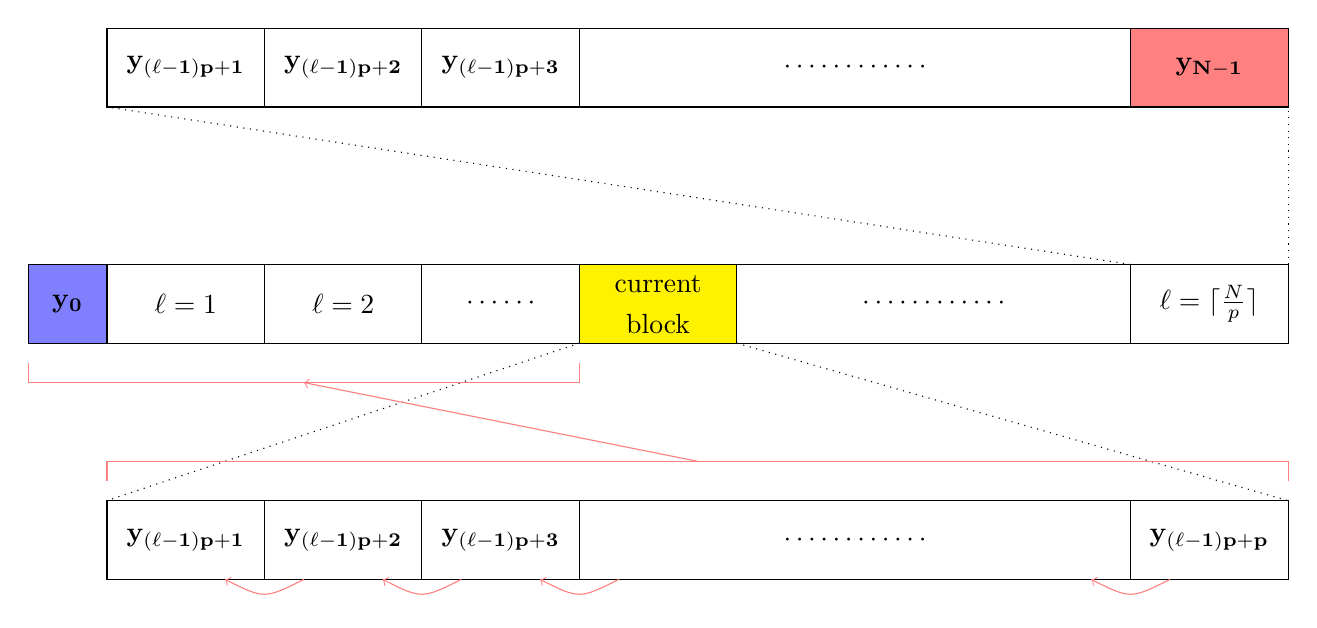
\begin{tikzpicture}
    \filldraw[fill=blue!50] (-1,0) rectangle (0,1);
    \draw (0,0) -- (0,1);
    \draw (-0.5,0.5) node { $ \mathbf{y_0} $ };
    \draw (-1,0) -- (15,0) -- (15, 1) -- (-1, 1) -- cycle;
    \draw (2,0) -- (2,1);
    \draw (4,0) -- (4,1);
    \draw (1,0.5) node { $ \ell = 1 $ };
    \draw (3,0.5) node { $ \ell = 2 $ };
    \draw (5,0.5) node { $ \cdots \cdots $ };
    \draw (6,0) -- (6,1);
    \draw (8,0) -- (8,1);
    \draw (10.5,0.5) node { $ \cdots \cdots \cdots \cdots  $ };
    \draw (13,0) -- (13,1);
    \draw (14,0.5) node { $ \ell = \lceil \frac{N}{p} \rceil $ };
    \filldraw[fill=yellow] (6,0) rectangle (8,1);
    \draw (7,0.75) node { current };
    \draw (7,0.25) node { block };
    \draw [dotted] (6,0) -- (0,-2);
    \draw [dotted] (8,0) -- (15,-2);
    \draw (0,-2) -- (15,-2) -- (15,-3) -- (0,-3) -- cycle;
    \draw (2,-3) -- (2,-2);
    \draw (4,-3) -- (4,-2);
    \draw (6,-3) -- (6,-2);
    \draw (13,-3) -- (13,-2);
    \draw (1,-2.5) node { $ \mathbf{ y_{(\ell - 1) p + 1} } $ };
    \draw (3,-2.5) node { $ \mathbf{ y_{(\ell - 1) p + 2} } $ };
    \draw (5,-2.5) node { $ \mathbf{ y_{(\ell - 1) p + 3} } $ };
    \draw (9.5, -2.5) node { $ \cdots \cdots \cdots \cdots $ };
    \draw (14,-2.5) node { $ \mathbf{ y_{(\ell - 1) p + p} } $ };
    \draw [dotted] (13,1) -- (0,3);
    \draw [dotted] (15,1) -- (15,3);
    \draw (0,3) -- (15,3) -- (15,4) -- (0,4) -- cycle;
    \draw (2,3) -- (2,4);
    \draw (4,3) -- (4,4);
    \draw (6,3) -- (6,4);
    \filldraw[fill=red!50] (13,3) rectangle (15,4);
    \draw (13,3) -- (13,4);
    \draw (1,3.5) node { $ \mathbf{ y_{(\ell-1)p + 1} } $ };
    \draw (3,3.5) node { $ \mathbf{ y_{(\ell-1)p + 2} } $ };
    \draw (5,3.5) node { $ \mathbf{ y_{(\ell-1)p + 3} } $ };
    \draw (9.5,3.5) node { $ \cdots \cdots \cdots \cdots $ };
    \draw (14,3.5) node { $ \mathbf{ y_{N-1} } $ };
    \draw [color=red!50, arrows={->}] (13.5,-3) .. controls (13,-3.25) .. (12.5,-3); 
    \draw [color=red!50, arrows={->}] (6.5,-3) .. controls (6,-3.25) .. (5.5,-3); 
    \draw [color=red!50, arrows={->}] (4.5,-3) .. controls (4,-3.25) .. (3.5,-3);    
    \draw [color=red!50, arrows={->}] (2.5,-3) .. controls (2,-3.25) .. (1.5,-3);
    \draw [color=red!50] (-1,-0.25) -- (-1,-0.5) -- (6,-0.5) -- (6,-0.25);
    \draw [color=red!50] (0,-1.75) -- (0,-1.5) -- (15,-1.5) -- (15,-1.75);
    \draw [color=red!50, arrows={->}] (7.5,-1.5) -- (2.5, -0.5);
\end{tikzpicture}

\caption{Computation diagram for the values in the vector (array) $ \mathbf{y} $.}
\label{fig:comp_diag}
\end{figure} 

The centre row shows how $ \mathbf{y} $ is broken up into blocks, and the bottom row is a detailed view
of the contents of the \emph{current block} being computed.

The red lines indicate dependency, in that $ \mathbf{y}_{(\ell - 1)p + 1} $ depends on all the $ y_j $ values calculated in the previous blocks. $ \mathbf{y}_{(\ell - 1)p + 2} $ depends on all the $ y_j $ values calculated in previous blocks \emph{and} on $ \mathbf{y}_{(\ell - 1)p + 1 } $. 

The idea is that in each block we can do all of the computations which only depend on previous blocks in parallel and then perform the calculations which are dependent on other values within the same block in sequence. After all the values in a particular block are calculated we move on to the next block and repeat the process.

An exploded view of the last block is also provided to emphasise the fact that this block might not contain $ p $ variables if $ p $ does not divide $ N - 1 $. This fact causes us no bother as it is easy to handle in code.

As in \cite{Diethelm2011} we rewrite the equations \eqref{eq:amb_y_corr} and $ \eqref{eq:amb_y_pred} $ as
\begin{align}
y_{j+1}^P = I_{j+1} + h^\alpha H_{j,\ell}^P + h^\alpha L_{j,\ell}^P
\end{align}
and
\begin{align}
y_{j+1} = I_{j+1} + h^{\alpha} H_{j,\ell} + h^\alpha L_{j,\ell}
\end{align}

where
\begin{align}
I_{j+1} & := \sum_{k=0}^{\lceil \alpha \rceil -1} \frac{x_{j+1}^k}{k!} y_0^{(k)} \\
H^P_{j,\ell} & := \sum_{k=0}^{(\ell-1)p} b_{j-k} f(x_k, y_k) \\
L_{j,\ell}^P & := \sum_{k=(\ell-1)p+1}^{j} b_{j-k} f(x_k,y_k) \\
H_{j,\ell} & := c_j f(x_0, y_0) + \sum_{k=1}^{(\ell - 1)p} a_{j-k}f(x_k, y_k) \\
L_{j,\ell} & := \sum_{k=(\ell-1)p + 1}^j a{j-k} f(x_k, y_k) + \frac{f(x_{j+1}, y^P_{j+1})}{\Gamma(\alpha + 2.)}
\end{align}

In each block the values of $ H, I $ and $ H^P $ can be calculated in parallel for each $ y_j $ in the block.Then there is a somewhat more complex dependency between these sums. 

To best explain how the processes procedes in each block and what dependencies there are we will consider a specific example where there are two values to be calculated per block (i.e. $ p = 2 $). Consider figure \ref{fig:AMB_Task_Flow}. 

Each box in the figure represents a task. A task can execute when all the tasks with arrows pointing to it have completed. The little red number represents the index of the variable \emph{within} the block which is being calculated. All the task names are reasonablly self explanatory except for perhaps $ S^P $ and $ S $. These take the values calculated in the other sums and add them together to get $ y^P $ and $ y $ respectivly. These are very small tasks which take very little time to execute.

The red arrow illustrate the interdependency of variables within a block. The second variable cannot have the sum $ L^P $ calculate until the first variable is calculated. This means that in effect each of the $ L $ tasks have to execute in series but these sums are relatively small so the time taken is quite short. Each block is then executed in sequence as each block depends on the blocks before it. See Appendix A for a C\# implementation of this. 

\begin{figure}[H]
%PID Controller Closed Loop Diagram.
\begin{tikzpicture} 
    \draw (10,20) -- (13,20) -- (13, 19) -- (10, 19) -- cycle;
    \draw (11.5,19.5) node { Block Start };
    \draw (11.5, 19) -- (11.5, 18);
    \draw (4.5, 18) -- (19.5, 18);
    \draw [->] (4.5, 18) -- (4.5, 17);
    \draw [->] (7.5, 18) -- (7.5, 17);
    \draw [->] (10.5, 18) -- (10.5, 17);
    \draw [->] (11.5, 18) -- (11.5, 13) -- (10, 13);
    \draw (3.75, 17) -- (5.25, 17) -- (5.25, 15.5) -- (3.75, 15.5) -- cycle;
    \draw (6.75, 17) -- (8.25, 17) -- (8.25, 15.5) -- (6.75, 15.5) -- cycle;
    \draw (9.75, 17) -- (11.25, 17) -- (11.25, 15.5) -- (9.75, 15.5) -- cycle;
    \draw (8.5, 12.25) -- (10, 12.25) -- (10,13.75) -- (8.5, 13.75) -- cycle;
    \draw (7.5, 14.5) -- (10.5, 14.5);
    \draw [->] (4.5, 15.5) -- (4.5, 4.25) -- (8.5, 4.25);
    \draw (7.5, 14.5) -- (7.5, 15.5);
    \draw (10.5, 14.5) -- (10.5, 15.5);
    \draw (7.5, 15.5) -- (7.5, 10);
    \draw [->] (7.5, 10) -- (8.5, 10);
    \draw (8.5, 9.25) -- (8.5, 10.75) -- (10, 10.75) -- (10, 9.25) -- cycle;
    \draw [->] (9.25, 12.25) -- (9.25, 10.75);
    \draw [->] (9.25, 9.25) -- (9.25, 8);
    \draw (8.5, 8) -- (10, 8) -- (10, 6.5) -- (8.5, 6.5) -- cycle ;
    \draw [->] (9.25, 6.5) -- (9.25, 5);
    \draw (8.5, 5) -- (8.5, 3.5) -- (10, 3.5) -- (10, 5) -- cycle;
    \draw [->] (18.5, 18) -- (18.5, 17);
    \draw [->] (15.5, 18) -- (15.5, 17);
    \draw [->] (12.5, 18) -- (12.5, 17);
    \draw (11.75, 17) -- (13.25, 17) -- (13.25, 15.5) -- (11.75, 15.5) -- cycle;
    \draw (14.75, 17) -- (16.25, 17) -- (16.25, 15.5) -- (14.75, 15.5) -- cycle;
    \draw (17.75, 17) -- (19.25, 17) -- (19.25, 15.5) -- (17.75, 15.5) -- cycle;
    \draw [->] (12.5, 15.5) -- (12.5, 4.25) -- (16.5, 4.25);
    \draw [->] (19.5, 18) -- (19.5, 13) -- (18, 13);
    
    
    \draw (15.5, 14.5) -- (18.5, 14.5);
    \draw [->] (12.5, 15.5) -- (12.5, 4.25) -- (16.5, 4.25);
    \draw (15.5, 14.5) -- (15.5, 15.5);
    \draw (18.5, 14.5) -- (18.5, 15.5);
    \draw (15.5, 15.5) -- (15.5, 10);
    \draw [->] (15.5, 10) -- (16.5, 10);
    \draw (16.5, 9.25) -- (16.5, 10.75) -- (18, 10.75) -- (18, 9.25) -- cycle;
    \draw [->] (17.25, 12.25) -- (17.25, 10.75);
    \draw [->] (17.25, 9.25) -- (17.25, 8);
    \draw (16.5, 8) -- (18, 8) -- (18, 6.5) -- (16.5, 6.5) -- cycle ;
    \draw [->] (17.25, 6.5) -- (17.25, 5);
    \draw (16.5, 5) -- (16.5, 3.5) -- (18, 3.5) -- (18, 5) -- cycle;
    \draw (16.5, 12.25) -- (18, 12.25) -- (18,13.75) -- (16.5, 13.75) -- cycle;
    \draw [color=red, arrows={->}] (10, 4.25) -- (12,4.25) -- (12, 13) -- (16.5, 13);
    \draw (4.5, 16.25) node { $ H $ };
    \draw (5, 15.75) node[color=red]  { $ 1 $ };
    
    \draw (7.5, 16.25) node { $ I $ };
    \draw (8, 15.75) node[color=red]  { $ 1 $ };
    
    \draw (10.5, 16.25) node { $ H_p $ };
    \draw (11, 15.75) node[color=red]  { $ 1 $ };
    
    \draw (9.25, 13) node { $ L_p $ };
    \draw (9.75, 12.5) node[color=red] { $ 1 $ };
    
    \draw (9.25, 10) node { $ S_p $ };
    \draw (9.75, 9.5) node[color=red] { $ 1 $ };
    
    \draw (9.25, 7.25) node { $ L $ };
    \draw (9.75, 6.75) node[color=red] { $ 1 $ };
    
    \draw (9.25, 4.25) node { $ L $ };
    \draw (9.75, 3.75) node[color=red] { $ 1 $ };
    
    
    
    \draw (12.5, 16.25) node { $ H $ };
    \draw (13, 15.75) node[color=red]  { $ 2 $ };
    
    \draw (15.5, 16.25) node { $ I $ };
    \draw (16, 15.75) node[color=red]  { $ 2 $ };
    
    \draw (18.5, 16.25) node { $ H_p $ };
    \draw (19, 15.75) node[color=red]  { $ 2 $ };
    
    \draw (17.25, 13) node { $ L_p $ };
    \draw (17.75, 12.5) node[color=red] { $ 2 $ };
    
    \draw (17.25, 10) node { $ S_p $ };
    \draw (17.75, 9.5) node[color=red] { $ 2 $ };
    
    \draw (17.25, 7.25) node { $ L $ };
    \draw (17.75, 6.75) node[color=red] { $ 2 $ };
    
    \draw (17.25, 4.25) node { $ L $ };
    \draw (17.75, 3.75) node[color=red] { $ 2 $ };
    
    \draw [->] (17.25, 3.5) -- (17.25, 2) -- (11.5, 2) -- (11.5, 1);
    
    \draw (10,1) -- (13,1) -- (13, 0) -- (10, 0) -- cycle;
    \draw (11.5,0.5) node { Block End };
\end{tikzpicture}

\caption{Task flow diagram for each block in the case when $ p = 2 $}
\label{fig:AMB_Task_Flow}
\end{figure}

\subsubsection{Analysis of the Performance of the Scheme in C\# and MONO}

We wish to analyse the performance of this scheme, and specifically its implementation in C\# (MONO). Although this scheme is extremely similar to that outlined in \cite{Diethelm2011} it differs mainly in the fact that this is a task based scheme which does not have an explicit number of threads which are executed. This is because we rely on a task scheduler to do that for us. In this scheme we let $ p $ denote the number of variables per block (and then spawn up to 4 simultaneous tasks per variable) instead of having $ p $ explicit threads for each block.

As can be seen from the code in Appendix A this results in easy to define dependencies and the bulk of the multithreading logic being done in just 40 lines of code.

A possible drawback of this scheme is that it relies on the a task scheduler which may or may not be optimised for the type of workload being placed on it. We will discuss this issue in more detail later on.

To understand the performance characteristics of this scheme see figure \ref{fig:mono_performance_surface} for a \emph{performance surface} which shows the average runtime of the scheme for different values of $ p $ and $ N $.

\begin{figure}[H]
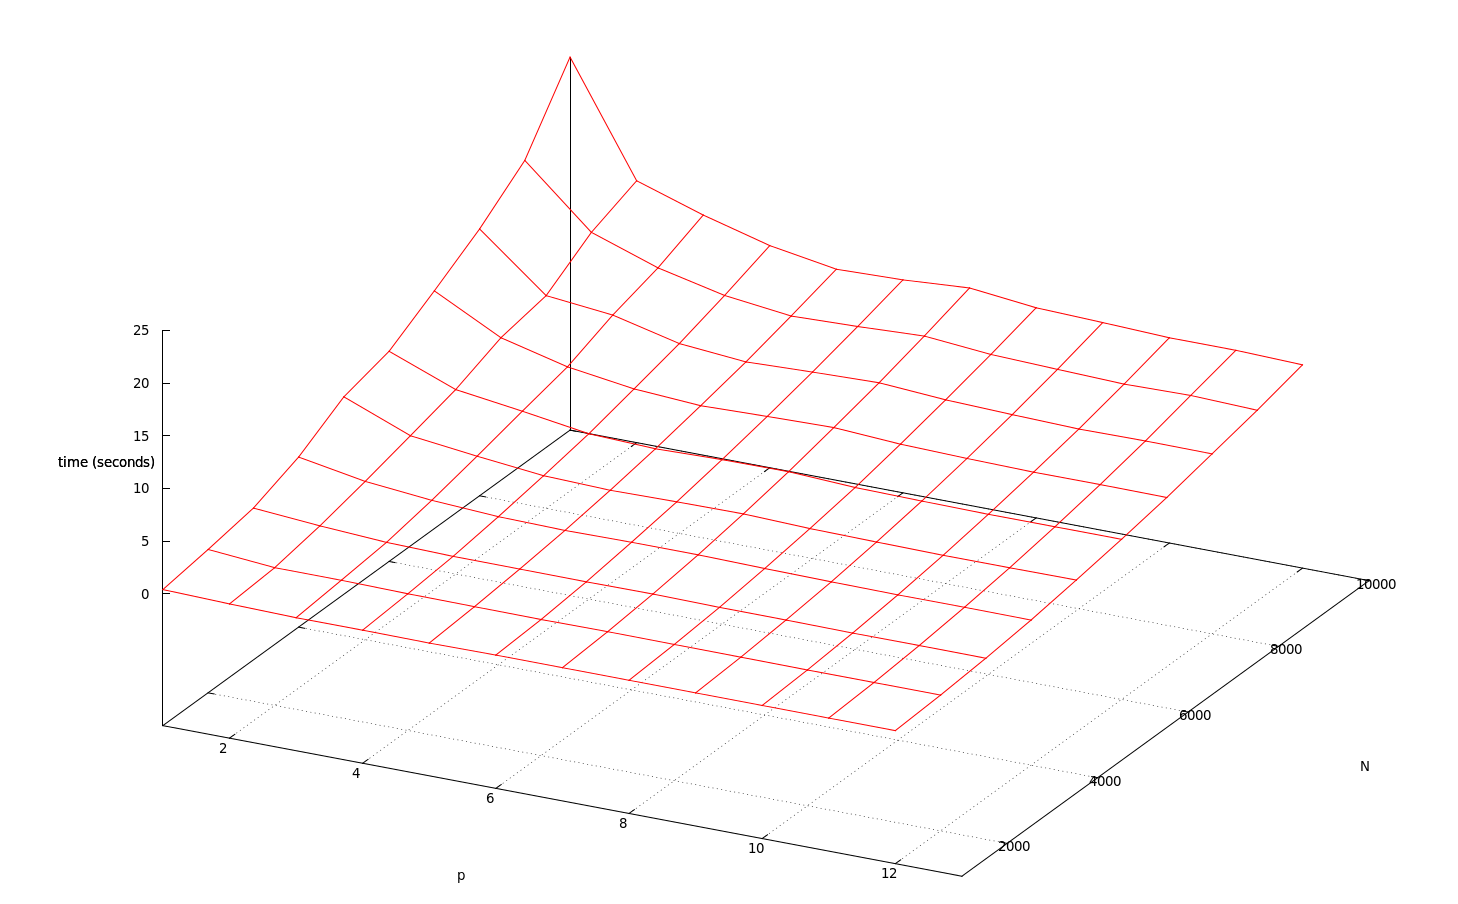
\includegraphics[scale = 0.3]{images/Dot_Net_Performance_No_Label}
\caption{Average runtime of the scheme for different values of $ p $ and $ N $}
\label{fig:mono_performance_surface}
\end{figure}

Firstly the $ O(N^2) $ complexity of the algorithm is quite clearly visible, especially in the case where $ p = 1 $. Secondly the law of diminishing returns is also clearly visible in this plot. In the case where $ p = 1 $ it should be noted that there are up to $ 4 $ tasks running just for that one variable ($ I $, $ L^P $, $ H $, $ H^P $). In \cite{Diethelm2011} $ p = 1 $ would refer to only 1 thread running at all times, which is not the case here. This is has its advantages and disadvantages. Its clearly advantageous because it results in potentially higher concurrency but disadvantageous because it limits out ability to compare this scheme with the one in \cite{Diethelm2011} on a \emph{thread for thread} basis.



\subsubsection{Parallelizing: A Naive CUDA Approach}
\label{sec:parallel_cuda}

\subsubsection{Reducing the Complexity Class: Speed - Accuracy Tradeoffs}
\label{sec:reduce_complexity}

\clearpage
